\documentclass[12pt,
a4paper,
openany,
oneside,
brazil,
]{abntex2}

\usepackage[brazil]{babel}
\usepackage[left=3cm,top=3cm,right=2cm,bottom=2cm]{geometry}
\usepackage{caption}
\usepackage{indentfirst}
\usepackage{graphicx}
\usepackage{xcolor}
\usepackage{microtype} 			% para melhorias de justificação
\usepackage[alf, 
  abnt-emphasize = bf,
  abnt-etal-list = 2,
  abnt-etal-cite = 2,
  bibjustif,
  abnt-etal-text=default
  % abnt-etal-text=it
  ]{abntex2cite}	% CITAÇÕES PADRÃO ABNT
\usepackage{fontspec}
\usepackage{url}
\setmainfont{Arial}

% O tamanho do parágrafo(recuo) é dado por:
\setlength{\parindent}{1.25cm}
\linespread{1.5}

\selectlanguage{brazil}

\makeatletter
\hypersetup{
      pdftitle={\@title}, 
		  pdfauthor={\@author},
	    pdfcreator={Hugo Soares},
      pdfkeywords={VLC}{Visible Light Communication}{SBC}{Dom Helder}{OpenVLC},
  		colorlinks=true,
    	citecolor=black,
      linkcolor=black,
      urlcolor=black,
	    bookmarksdepth=4
}

\renewcommand\printchaptertitle[1]{%
    \chaptitlefont%
    \ifthenelse{\boolean{abntex@innonumchapter}}{\ABNTEXchapterupperifneeded{#1}}{%
    \ifthenelse{\boolean{abntex@apendiceousecao}}{%
        \centering%
        \settowidth{\chapternamenumlength}{\printchaptername\printchapternum\afterchapternum}%
        \ABNTEXchapterupperifneeded{#1}%
      }{%
        \settowidth{\chapternamenumlength}{\printchaptername\printchapternum\afterchapternum}%
        \parbox[t]{\columnwidth-\chapternamenumlength}{\ABNTEXchapterupperifneeded{#1}}}%
     }   
}

\captionsetup{justification=raggedright,singlelinecheck=false}

\titulo{Comunicação por luz visível: \\ Construindo um protótipo usando SBC e explorando o potencial da tecnologia VLC}
\autor{Hugo Oliveira Soares}
\local{Belo Horizonte}
\instituicao{DOM HELDER ESCOLA SUPERIOR}
\orientador{Prof. Marden Cicarelli Pinheiro}
\coorientador{Prof. Ricardo Luiz de Freitas}
\preambulo{
  Projeto de Pesquisa apresentado à Dom Helder Escola Superior como requisito parcial para obtenção do título de Cientista da Computação.
  \newline 
  \newline
  Orientador de conteúdo: \imprimirorientador
  \newline
  \newline
  Orientador de metodologia: \imprimircoorientador
}
\data{2023}

\begin{document}

  % PARTE PRÉ-TEXTUAL
  \pagenumbering{roman}
  \pretextual
  \renewcommand{\imprimircapa}{
  \begin{capa}
    \center

    \begin{center}
      {\ABNTEXchapterfont\bfseries\LARGE\imprimirtitulo}
    \end{center}

    \vspace*{2cm}

    {\ABNTEXchapterfont\large\imprimirautor\footnote{Graduando em Ciência da Computação, Escola Superior Dom Helder, \href{mailto:e01381@ academico.domhelder.edu.br}{e01381@academico.domhelder.edu.br}}}
    \\
    {\ABNTEXchapterfont\large\imprimirorientador\footnote{Mestre em Tecnologia da informação(CEFET), docente do curso Ciência da Computação, Escola Superior Dom Helder Câmara, marden.cicarelli@academico.domhelder.edu.br}}
    \\
    {\ABNTEXchapterfont\large\imprimircoorientador\footnote{Mestre em Administração (FUMEC), docente do curso de Ciência da Computação, Escola Superior Dom Helder, \href{mailto:ricardo.freitas@academico.domhelder.edu.br}{ricardo.freitas@academico.domhelder.edu.br}}}

     \vspace{\onelineskip}
     \vspace{\onelineskip}

     % RESUMO
     \begin{flushleft}
      {\ABNTEXchapterfont\bfseries\large Resumo}

      \justifying O \textit{Visible Light Communication} (VLC) é uma tecnologia que utiliza o espectro da luz visível para a transmissão de dados. Com o aumento da popularidade da internet e do uso de dispositivos IoT, a demanda por redes wifi tem crescido exponencialmente, causando congestão nas faixas de espectro eletromagnético destinadas a essas redes. O VLC surge como uma solução promissora para este problema, aproveitando as diversas faixas de frequência disponíveis na luz visível. Além disso, o VLC evita interferências eletromagnéticas em dispositivos eletrônicos e redes wifi. O estudo demonstrou a viabilidade da implementação do sistema VLC com a \textit{Single Board Computer} (SBC) \textit{OrangePi}, tendo como resultado um protótipo bem sucedido em realizar uma transmissão de dados.
      \vspace{\onelineskip}
 
      \noindent
      \textbf{Palavras-chave}: Protótipo. Comunicação por luz visível. VLC. SBC. OpenVLC. \textit{RaspberryPi}. \textit{OrangePi}
    \end{flushleft}

    \vspace{\onelineskip}

  \end{capa}
}


 
  \imprimircapa
  \clearpage
  \makeatletter
\renewcommand{\folhaderostocontent}{
  \begin{center}

    {\ABNTEXchapterfont\large\imprimirautor}

    \vspace*{\fill}
    \begin{center}
      \ABNTEXchapterfont\bfseries\Large\imprimirtitulo
    \end{center}

    \vspace*{\fill}

    \abntex@ifnotempty{\imprimirpreambulo}{
      \hspace{.45\textwidth}
      \begin{minipage}{.5\textwidth}
          \SingleSpacing
          \ABNTEXfontereduzida
          \imprimirpreambulo
      \end{minipage}
      \vspace*{\fill}
    }


    \vspace*{\fill}

    \imprimirlocal
    \par
    \imprimirdata
    \vspace*{1cm}

    \end{center}
}
\makeatother

  \imprimirfolhaderosto

  \listoffigures % Lista de imagens
  % \begin{siglas}

  \item[IOT]  Internet Of Things
  \item[VLC]  Visible Light Communication  

\end{siglas}
 % Lista de abreviaturas e siglas
  \clearpage
  \tableofcontents %SUMARIO
  % \clearpage

  % PARTE TEXTUAL
  \pagenumbering{arabic}
  \textual
  %% CAPITULOS
  \chapter{Introdução}

Com o aumento da popularidade da internet em todo o mundo, é notável que as redes \textit{wifi} têm crescido significativamente, juntamente com o número de usuários e de dispositivos IoT (Internet Of Things) \cite{matheus2017comunicaccao}. De acordo com o relatório Digital 2023: Global Overview Report, publicado pelo site Datareportal, há cerca de 5,16 bilhões de usuários na internet. No entanto, esse aumento na demanda por \textit{wifi} tem causado um problema, que é a congestão das faixas do espectro eletromagnético reservadas para essas redes, assim afetando a sua eficiência.

\begin{figure}[!htbp]
  \caption{Indicadores de uso da Internet}
  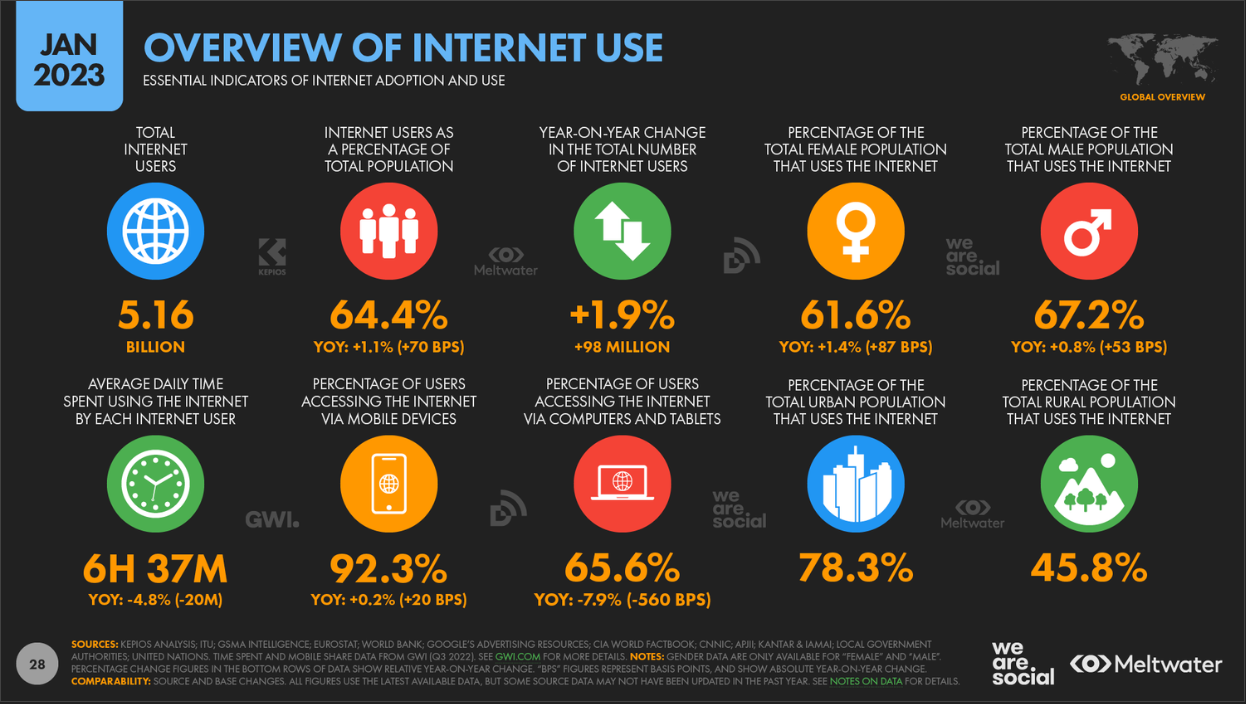
\includegraphics[scale=0.4]{images/internet_use.png}
  \legend{Fonte: \citeonline{datareportal}}
  \label{figura:usoInternet}
\end{figure}

As redes \textit{wireless} utilizam ondas eletromagnéticas para a transmissão de dados e informações, o que inviabiliza ou dificulta a sua utilização em alguns lugares, como em hospitais e aeronaves, por exemplo, por interferir com equipamentos hospitalares e com a antena de transmissão no caso dos voos.

Diante desses cenários, o \textit{Visible Light Communication} (VLC) se mostra como um forte candidato para a solução destes problemas.
Verifica-se que o espectro da luz visível, possui 10 mil vezes mais faixas de frequência se comparado com as ondas de rádio \cite[p. 14]{conceiccao2015comunicaccao}.
Ou seja, é possível que um único ``roteador” se comunique com mais dispositivos ao mesmo tempo.

Para o problema de interferência o VLC também é uma solução, visto que utiliza a luz visível como forma de transmitir as informações, assim não gerando interferências eletromagnéticas em outros aparelhos eletrônicos ou em redes \textit{wifi}.

O estudo objetiva verificar a viabilidade de implementação do sistema VLC com um \textit{SBC (Single Board Computer)}, através da construção de um protótipo. A pesquisa experimental surgiu da necessidade de uma nova forma de transmissão de dados com pouca interferência e de baixo custo, abrindo uma  possibilidade de levar comunicação em locais onde não era possível recorrer a uma rede \textit{wireless}.


  \chapter{Objetivos}
\section{Objetivo geral}

O propósito desta pesquisa é a construção de um protótipo de um sistema de comunicação VLC, baseado no projeto OpenVLC, utilizando o mini-computador Raspberry Pi. O objetivo principal é que o sistema seja capaz de transmitir e receber alguns bytes.

\section{Objetivos específicos}

\begin{itemize}

  \item Explicar o funcionamento do VLC
  \item Pesquisar as vantagens e desvantagens
  \item Implementar um protótipo
  \item Avaliar o desempenho do protótipo

\end{itemize}


  \chapter{Justificativa}

Segundo o autor \citeauthoronline{tanenbaum} o comitê do IEEE definiu que as redes no padrão 802.11, \textit{wifi}, utilizariam as frequências de 2,4GHz e 5GHz e que todos os dispositivos têm a permissão para utilizá-los desde que limitem a sua potência para permitir que dispositivos diferentes coexistam. O autor \citeonline{barros} também cita que há muitos outros equipamentos eletrônicos que geram ondas também na faixa de 2,4GHz. 

Devido a faixa de 2,4GHz ser internacionalmente regulamentada ela não necessita de licença para a sua utilização e com a popularidade das redes sem fio a faixa tem concentrado grande parte da demanda por frequência. Assim o seu compartilhamento tem se tornado bastante denso fazendo com que os receptores lidem constantemente com interferências \cite{barros}. Segundo \citeonline{fcc} o problema do congestionamento do espectro é crescente e está cada vez mais comum nas residências.

Outro problema enfrentado pelas redes sem fio é a interferência eletromagnética gerada por dispositivos elétricos que pode afetar o funcionamento da comunicação e vice-versa, como por exemplo um forno de microondas. Esses aparelhos operam na faixa de 2,45GHz, assim provocando um aumento nas taxas de erro nos dados que trafegam nas redes \cite{barros}. Já no caso contrário as redes móveis podem provocar alterações no funcionamento de dispositivos hospitalares e colocar em risco a vida dos pacientes \cite{cabral}.

A construção de um protótipo de um sistema VLC se dá pelo seu grande potencial de solucionar os problemas citados acima. Como o VLC utiliza uma faixa de comprimento de onda que vai de cerca de 380nm até 780nm, permite que a tecnologia ofereça uma faixa de frequências cerca de 10 mil vezes maior do que a radiofrequência, permitindo que mais dispositivos se conectem no mesmo ponto de acesso assim solucionando o problema do congestionamento do espectro \cite{conceiccao2015comunicaccao}. 

Como a luz visível não interfere em equipamentos eletrônicos, o VLC tem a possibilidade de operar  em locais onde a RF não é desejada, como por exemplo em hospitais, evitando o mau funcionamento dos dispositivos.


  \section{Referencial teórico}  

\subsection{Padrão IEEE 802.11}

Quando os computadores receberam transmissores e receptores de rádio varias empresas começaram a comercializar LANs sem fios, porém não havia uma padronização para a comunicação, ou seja, um computador equipado com um rádio da marca \emph{X} não era compatível com o computador equipado com o rádio da marca \emph{Y}. Diante deste problema surgiu a necessidade de se criar um padrão para as LANs sem fios, assim o comitê do IEEE criou o padrão 802.11 mais conhecido como \textit{wifi} \cite{tanenbaum}.

\subsubsection{Faixas 2.4Ghz e 5Ghz}

As faixas de radio que o \textit{wifi} utiliza são as faixas de 2,4GHz e 5GHz, as duas bandas não necessitam de licença para a sua utilização contudo os aparelhos devem limitar a sua potência para permitir que diferentes dispositivos coexistam \cite{tanenbaum}. Como a utilização da faixa é livre é muito provável que os equipamentos de \textit{wifi} tenham que lidar constantemente com interferências. 

\subsection{Interferência eletromagnética}

\subsection{OpenVLC}

  \chapter{Metodologia}

Segundo \citeonline{wiltgen2019prototipos}, um protótipo é uma representação similar ao produto a ser desenvolvido, criado com o intuito de realizar testes e ensaios para que as funcionalidades se comportem como esperado no ambiente de uso. Nesse contexto, o objetivo principal deste trabalho é implementar um protótipo de um sistema VLC utilizando um SBC como plataforma de desenvolvimento. Durante o desenvolvimento foram utilizados elementos de metodologias ágeis como os do \textit{Scrum} e do \textit{Kanban}.

O \textit{Scrum} é uma estrutura que define diversos eventos como as \textit{sprints} que são ciclos de desenvolvimento com um tempo definido, geralmente de duas semanas, e a retrospectiva que é o momento em que a equipe discute o que foi bom ou ruim no ciclo (\textit{sprint}) que se passou. O \textit{Scrum} também define os membros da equipe e suas responsabilidades, como o PO, o \textit{Scrum Master} e a equipe de desenvolvimento \cite{scrum}. 

O \textit{Kanban} é uma estrutura que permite a visualização dos itens de trabalho que são organizados em um quadro que é dividido em \textit{To Do}, \textit{In Progress} e \textit{Done} \cite{kanbam}.

Para a avaliação do desempenho das SBCs selecionadas foram coletadas as informações de uso do processador, o uso de memória RAM e também a taxa de erros durante a transmissão de um pacote de dados.

\section{Single Board Computer (SBC)}

\textit{Single Board Computer} (SBC) é um computador onde todos os componentes necessários estão em uma mesma placa de circuito impresso. Esse tipo de dispositivo é muito utilizado para fins educacionais, para desenvolvimento de sistemas, datacenters (centros  de  processamento  de  dados) e clusters portáteis. Alguns exemplos são o \textit{OrangePI}, \textit{RockPI}, \textit{BeagleBone} e \textit{RaspberryPI}, sendo este um dos mais populares \cite{SBC_edu}.

Os SBCs geralmente são de baixo custo, porém devido a escassez global de semicondutores reduziu a sua disponibilidade e por consequência levou ao aumento dos preços \cite{zeng_2022}. Principalmente do \textit{RaspberryPI} que passou de 45 dólares para 161 dólares, por esse motivo o SBC \textit{OrangePI} foi selecionado para o desenvolvimento deste trabalho.

\subsection{RaspberryPI}

A \textit{Raspberry Pi Foundation} foi fundada em 2008 sediada no Reino Unido com o objetivo de promover o avanço na educação no campo da computação. \cite{rasp}

O \textit{RaspberryPI} é um pequeno computador que traz consigo um processador na arquitetura ARM, a mesma tecnologia que se encontra em num smartphone \cite{rasp}.\newline

\begin{figure}[!htbp]
  \caption{Raspberry Pi 3}
  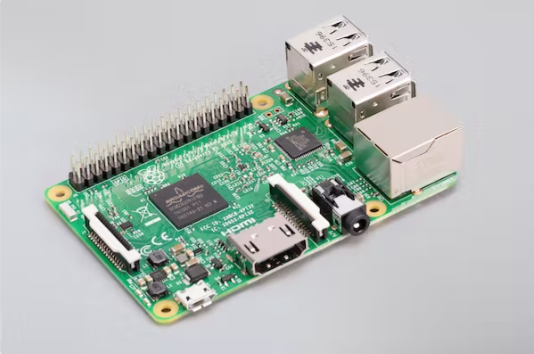
\includegraphics[scale=0.4]{images/rasp.png}
  \legend{Fonte: \citeonline{rasp}}
  \label{figura:rasp}
\end{figure}

\subsection{OrangePI}

O \textit{OrangePI} é um SBC \textit{open source} da Shenzhen Xunlong Software. A arquitetura de seu processador é ARM e a plataforma suporta vários sistemas operacionais como Android e as várias distribuições de linux \cite{orangepi}.\newline

\begin{figure}[!htbp]
  \caption{Orange Pi 3 LTS}
  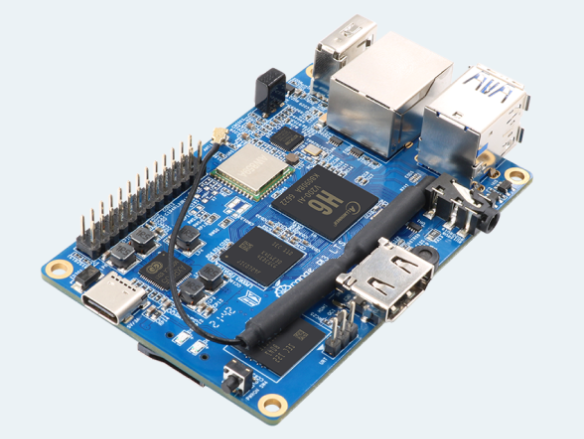
\includegraphics[scale=0.35]{images/orange.png}
  \legend{Fonte: \citeonline{orangepi}}
  \label{figura:orange}
\end{figure}

\newpage

\subsection{BeagleBone Black}

\textit{BeagleBone Black} é uma plataforma suportada pela comunidade que roda Linux para prototipagem rápida \cite{beaglebone}.
Esta plataforma é utilizada pelo projeto OpenVLC. \newline

\begin{figure}[!htbp]
  \caption{BeagleBone Black}
  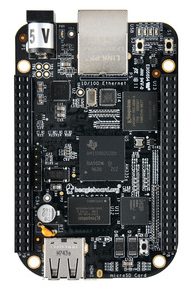
\includegraphics[scale=0.58]{images/beaglebone.png}
  \legend{Fonte: \citeonline{beaglebone}}
  \label{figura:beagle}
\end{figure}

\section{Linux}

Linux é um sistema operacional de computadores, o autor \citeonline{negus} cita em seu livro Linux a Bíblia que este sistema é um exemplo de como projetos colaborativos podem ultrapassar o que empresas individuais podem fazer.

O Linux permite que os desenvolvedores alterem o sistema como quiserem ajudando a criar softwares para as suas necessidades, por esse motivo utilizaremos este sistema no desenvolvimento do trabalho.

  \chapter{Resultados esperados}

É esperado deste trabalho que contribua no entendimento dos processos para a realização dos objetivos declarados no capítulo \ref{obj}, além de auxiliar a compreender mais sobre a tecnologia VLC e o que ela pode trazer de benefícios para a sociedade.

Que as informações deste trabalho possam ser úteis e que ao mesmo tempo incentive outros pesquisadores a desenvolverem projetos sobre o tema, já que foi utilizado uma SBC mais acessível para o cenário brasileiro.

  \section{Desenvolvimento}

Este capítulo detalha os processos que ocoreram no desenvolvimento da pesquisa, mostrando os passos seguidos para alcançar os objetivos propostos. Além disso, são abordadas as dificuldades enfrentadas e as adptações e refinamentos realizados ao longo do percurso.

\subsection{Circuito}

\subsubsection{Emissor}

O circuito que permite ``transformar" os bits em luz é composto por um led de alto brilho, um transistor TIP122, dois resistores e uma bateria.

O transistor é ligado como chave na SBC para permitir acionar cargas elétricas da qual a SBC não seria capaz, pois pode fornecer no máximo 16 mA (miliampère) \citeonline{correnteSbc} e como o \textit{led} de alto brilho consome uma corrente de 18.8mA, uma ligação direta na GPIO (\textit{General Purpose Input/Output}) poderia queimar a SBC.

\begin{figure}[!htbp]
  \caption{Esquema do circuito emissor}
  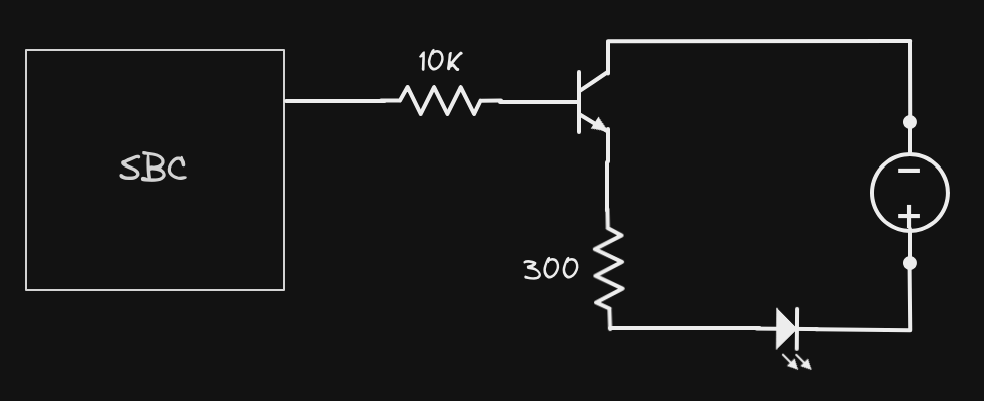
\includegraphics[width=0.5\textwidth]{images/esquema_circuito_emisor.png}
  \legend{Fonte: Autor (2023)}
  \label{esquema-circuito-emissor}
\end{figure}

\begin{figure}[!htbp]
  \caption{Foto do circuito emissor}
  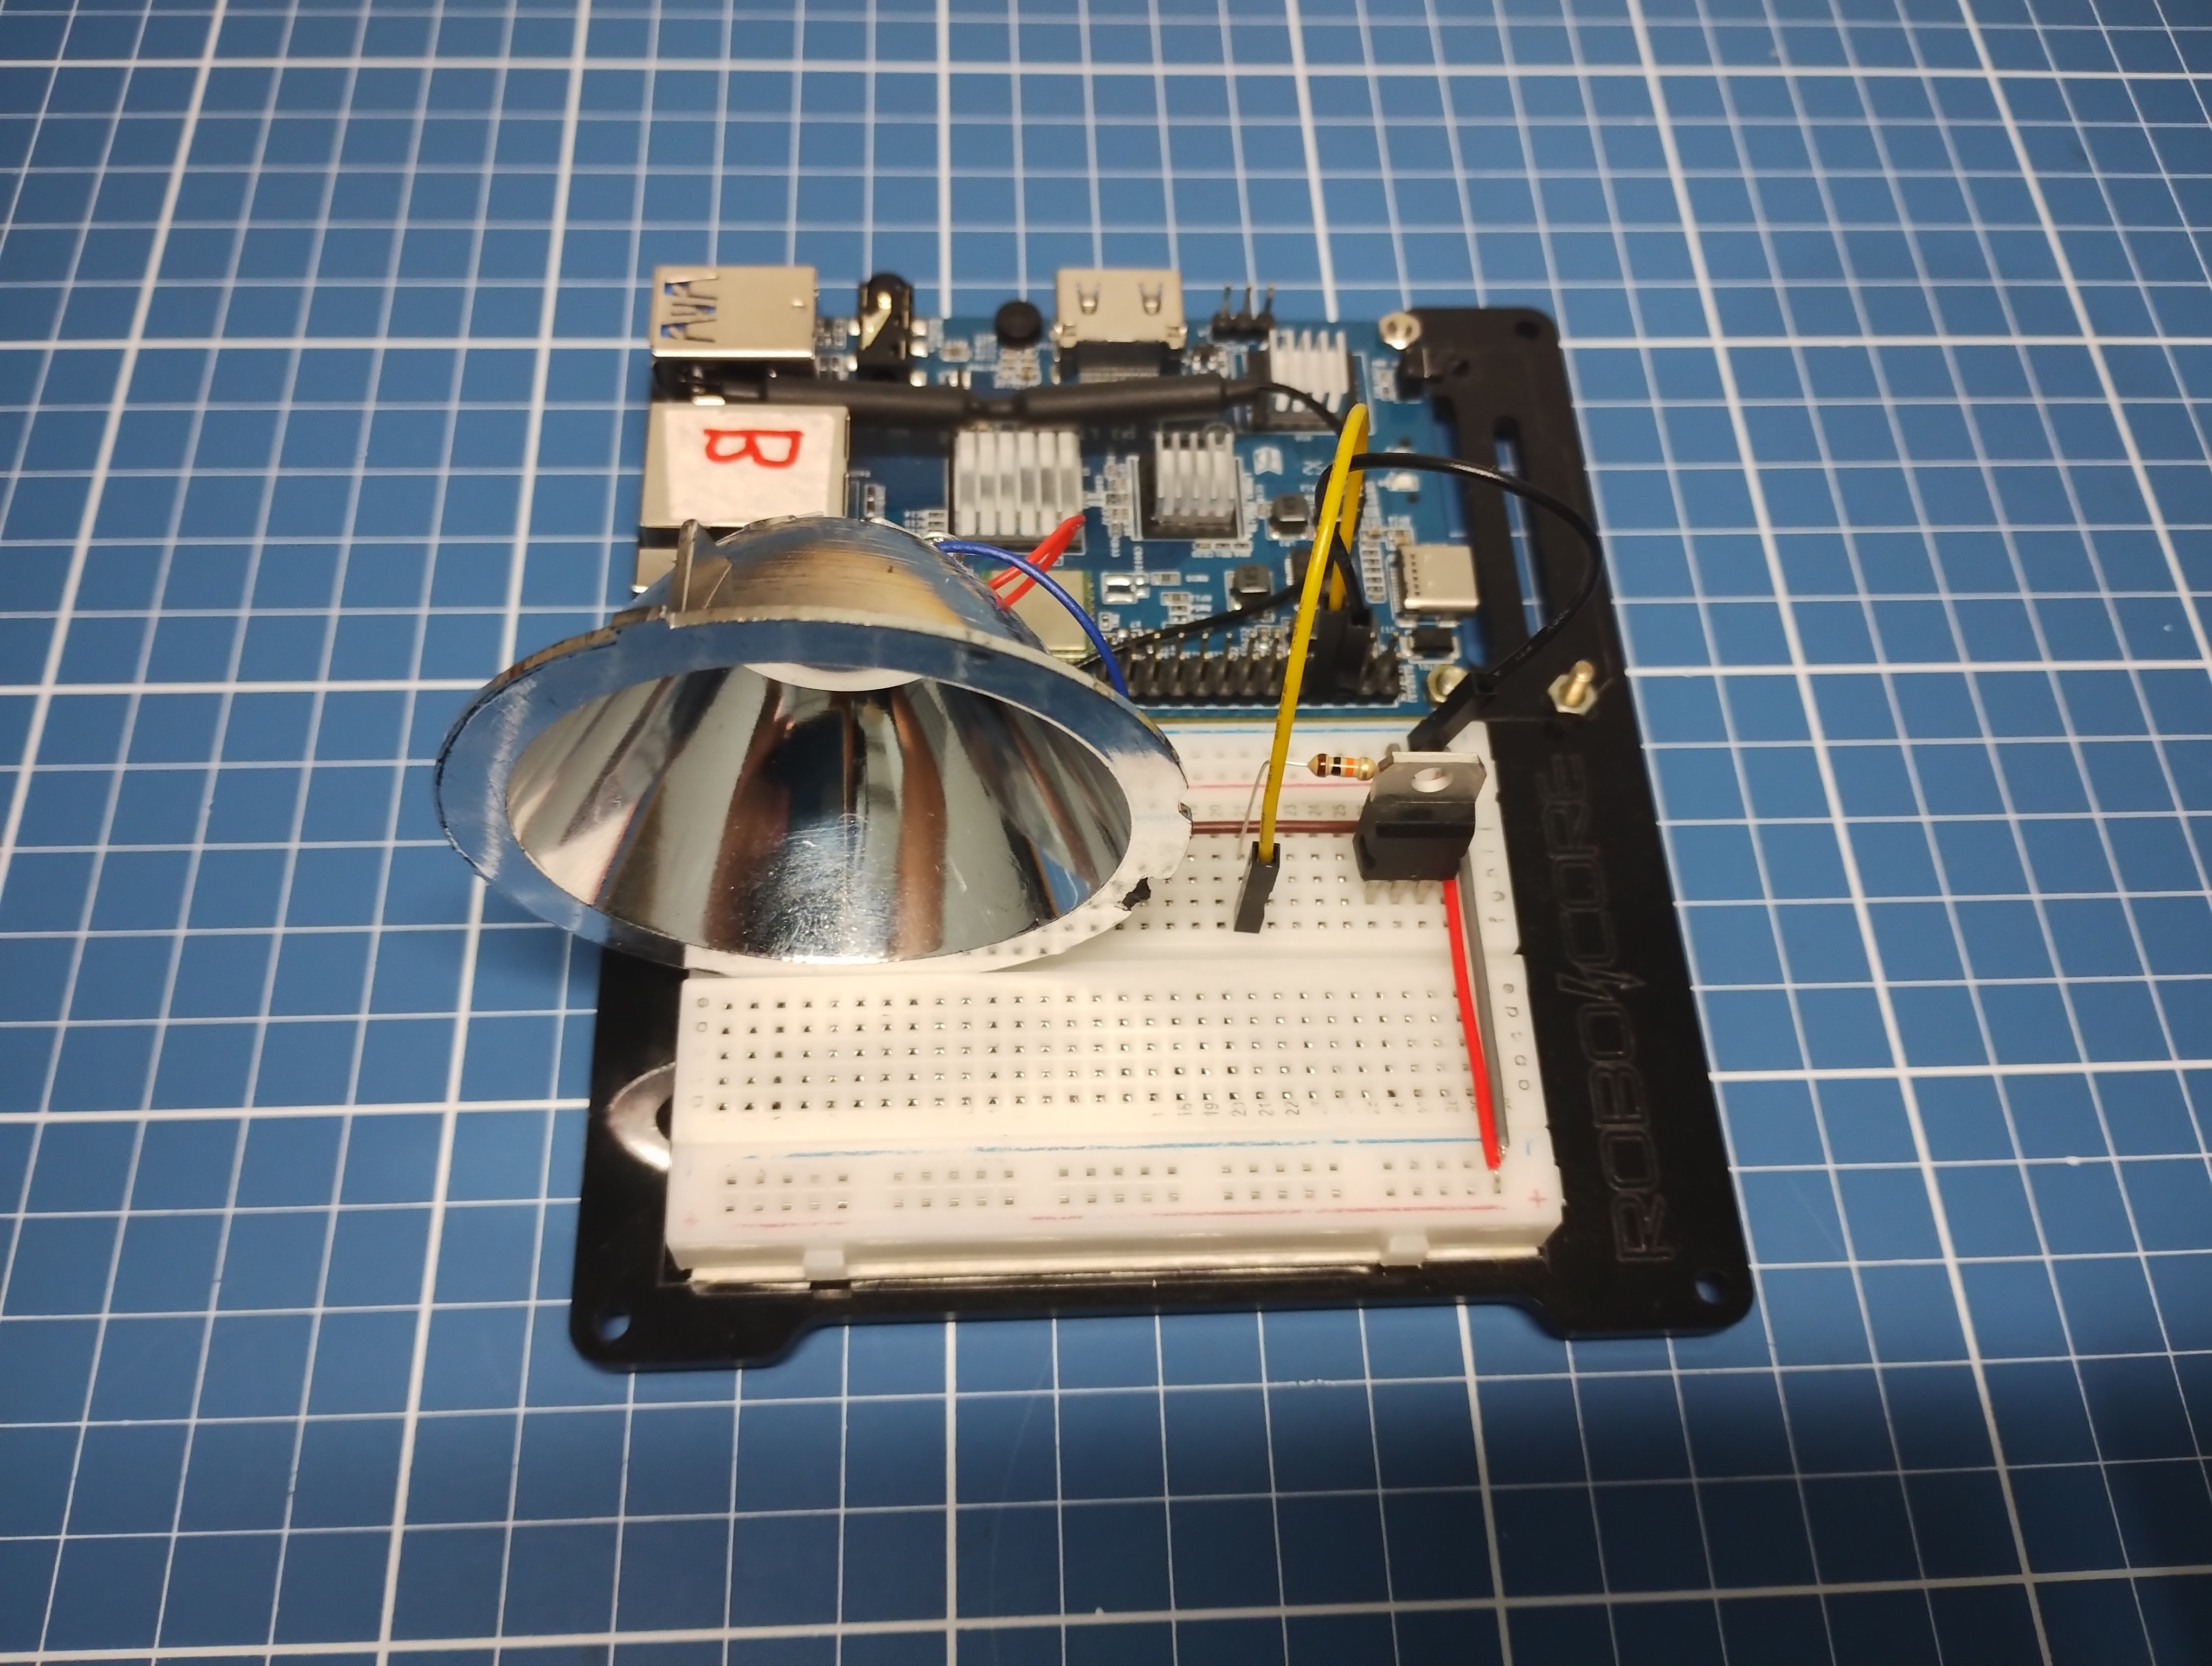
\includegraphics[width=0.4\textwidth]{images/foto_circuito_emisor.jpg}
  \legend{Fonte: Autor (2023)}
  \label{foto-circuito-emissor}
\end{figure}

\begin{figure}[!htbp]
  \caption{Consumo do \textit{led} usado no circuito emissor}
  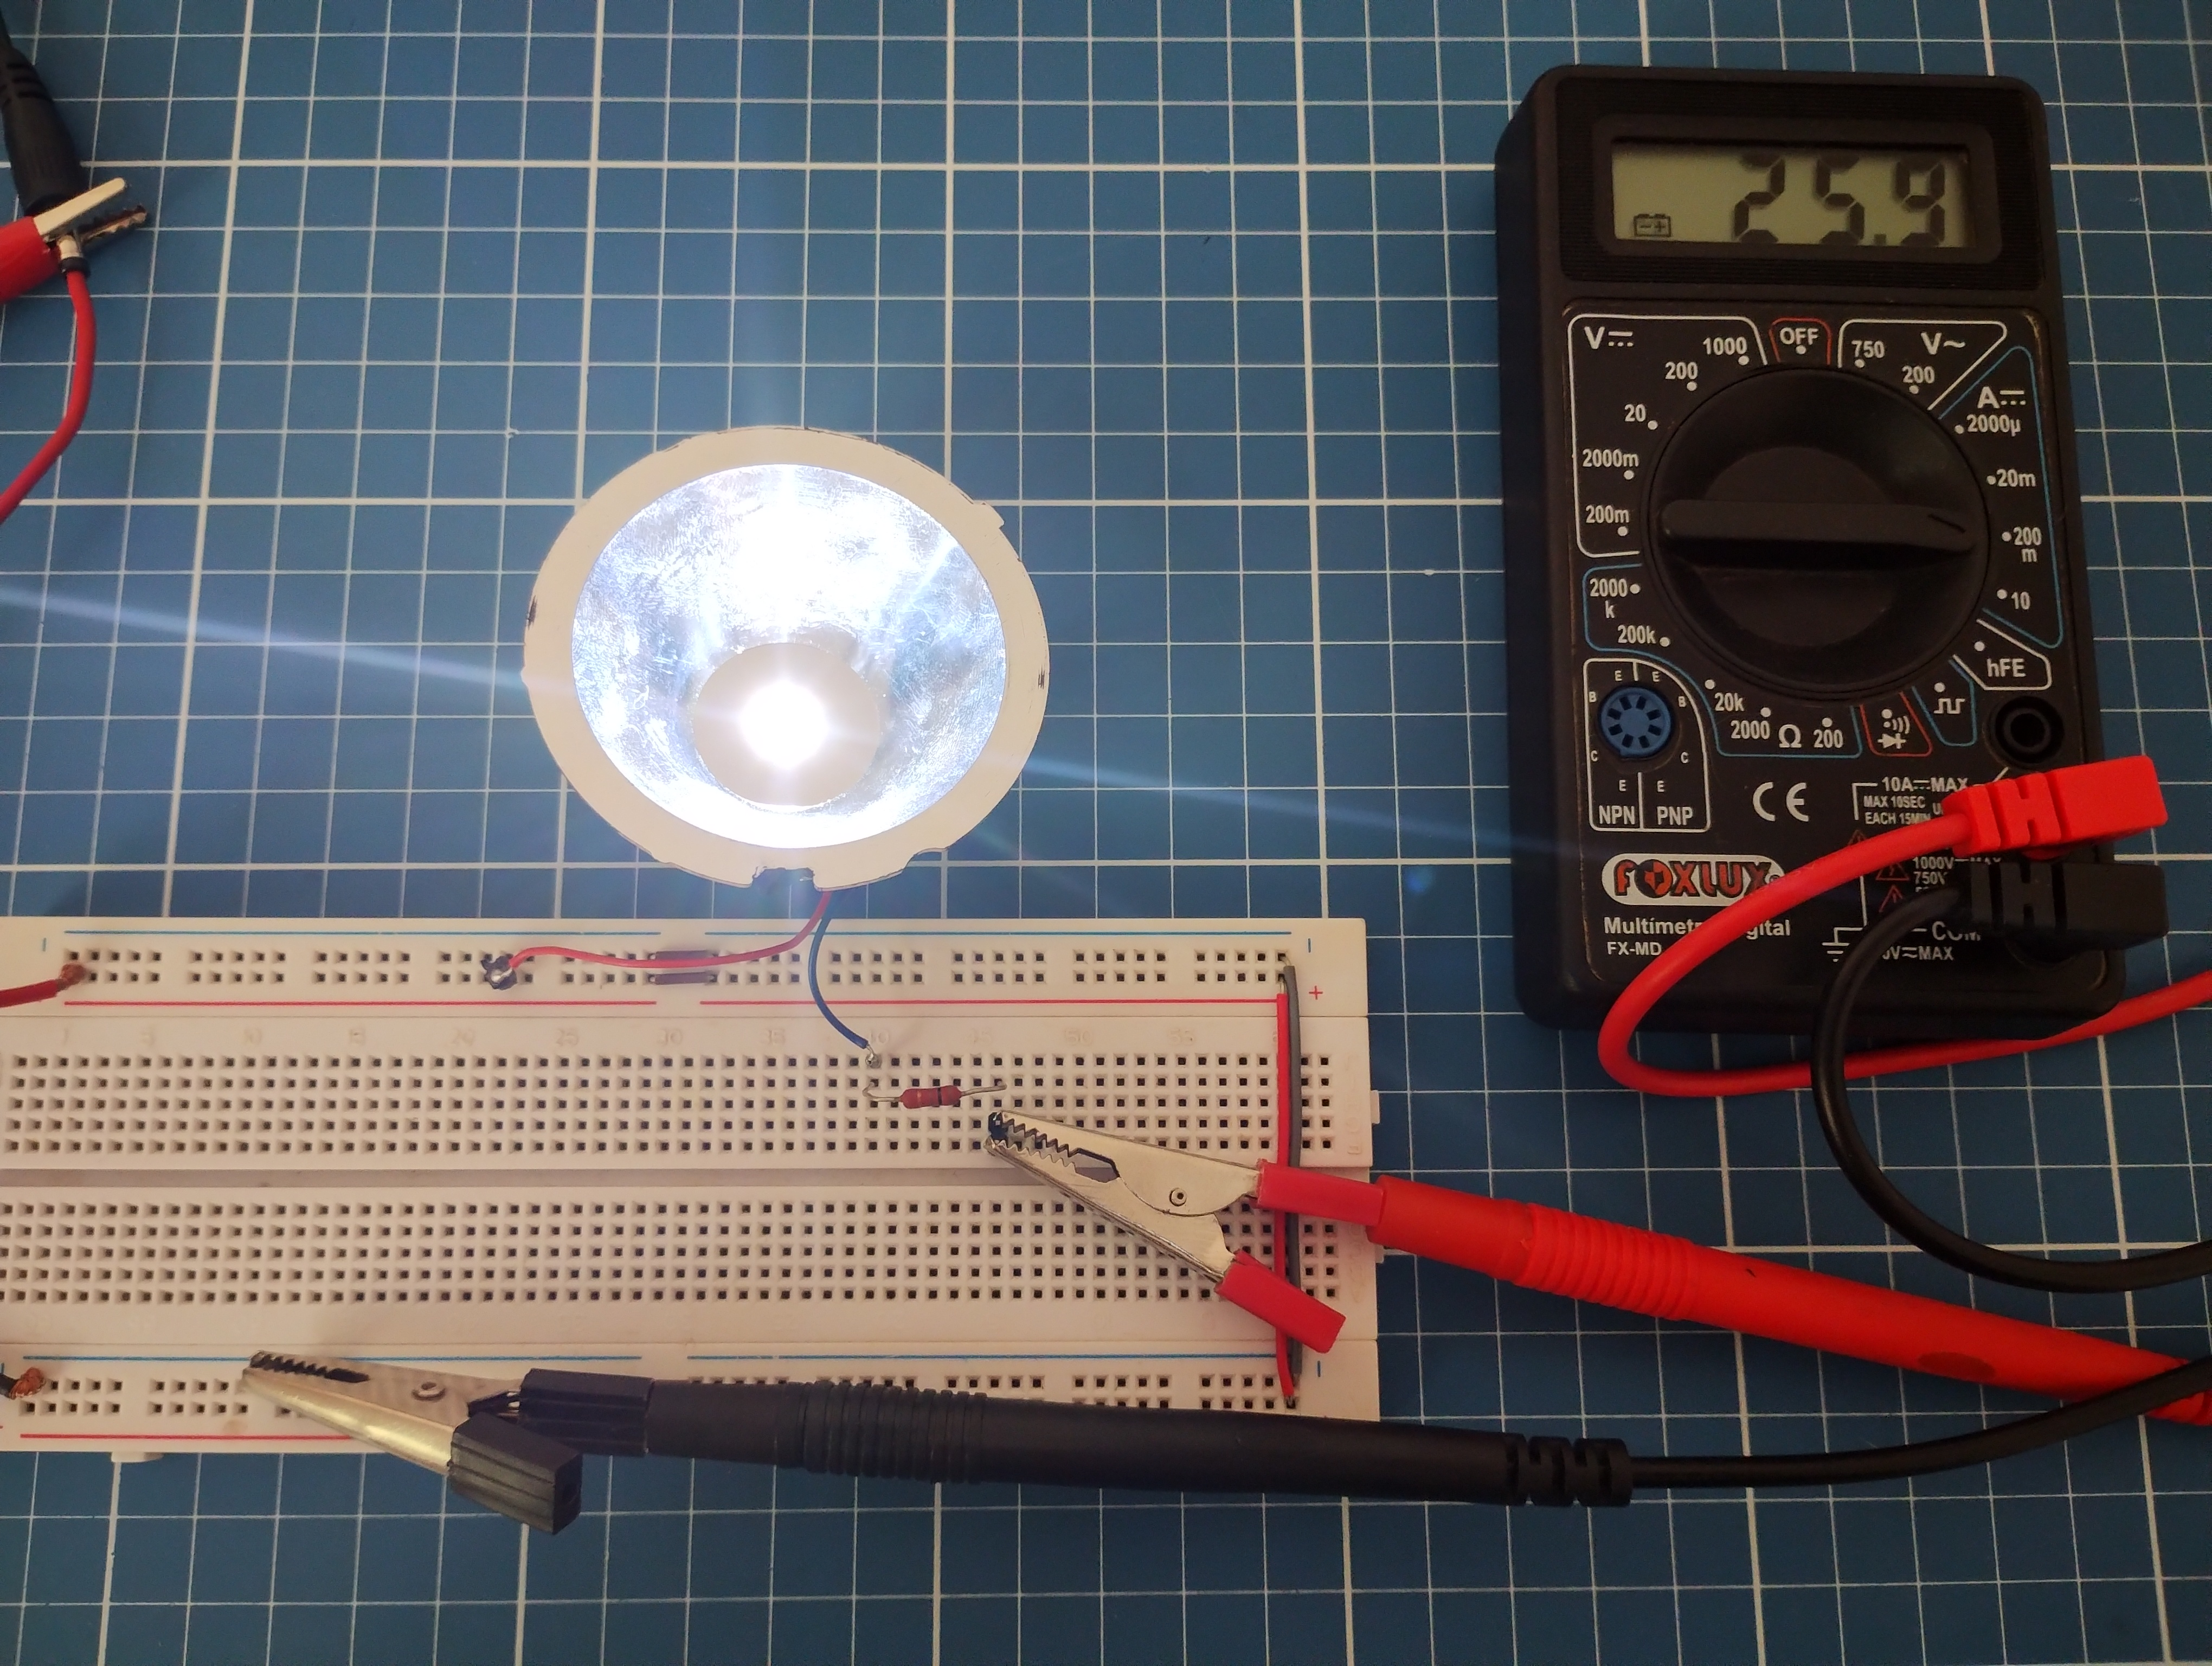
\includegraphics[width=0.4\textwidth]{images/consumo_led.jpg}
  \legend{Fonte: Autor (2023)}
  \label{corrente_led}
\end{figure}


\subsubsection{Receptor}

O circuito para receber as informações do emissor é composto por um LDR (\textit{Light Dependent Resistor}) e um potenciômetro ligado em série. Este circuito permite estabelecer uma faixa de corte de acordo com o nível de luminosidade do ambiente.

Estabelecido a faixa de corte ajustando o potenciômetro é possível "perceber" quando se está em nível lógico alto (bit 1) ou em nível lógico baixo (bit 0).


\begin{figure}[!htbp]
  \caption{Esquema do circuito receptor}
  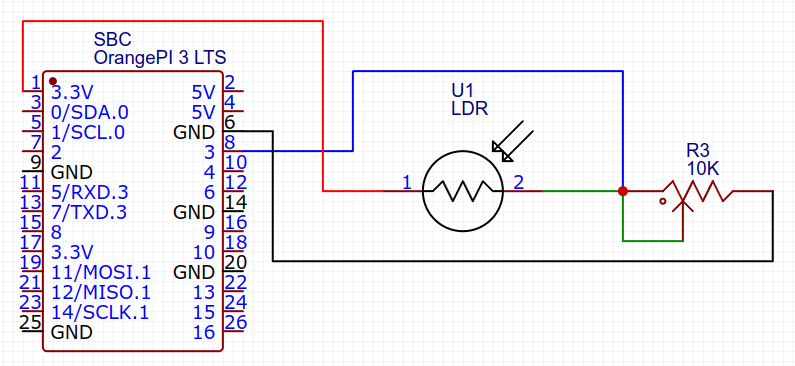
\includegraphics[width=0.5\textwidth]{images/esquema_circuito_receptor.png}
  \legend{Fonte: Autor (2023)}
  \label{esquema-circuito-receptor}
\end{figure}


\begin{figure}[!htbp]
  \caption{Foto do circuito receptor}
  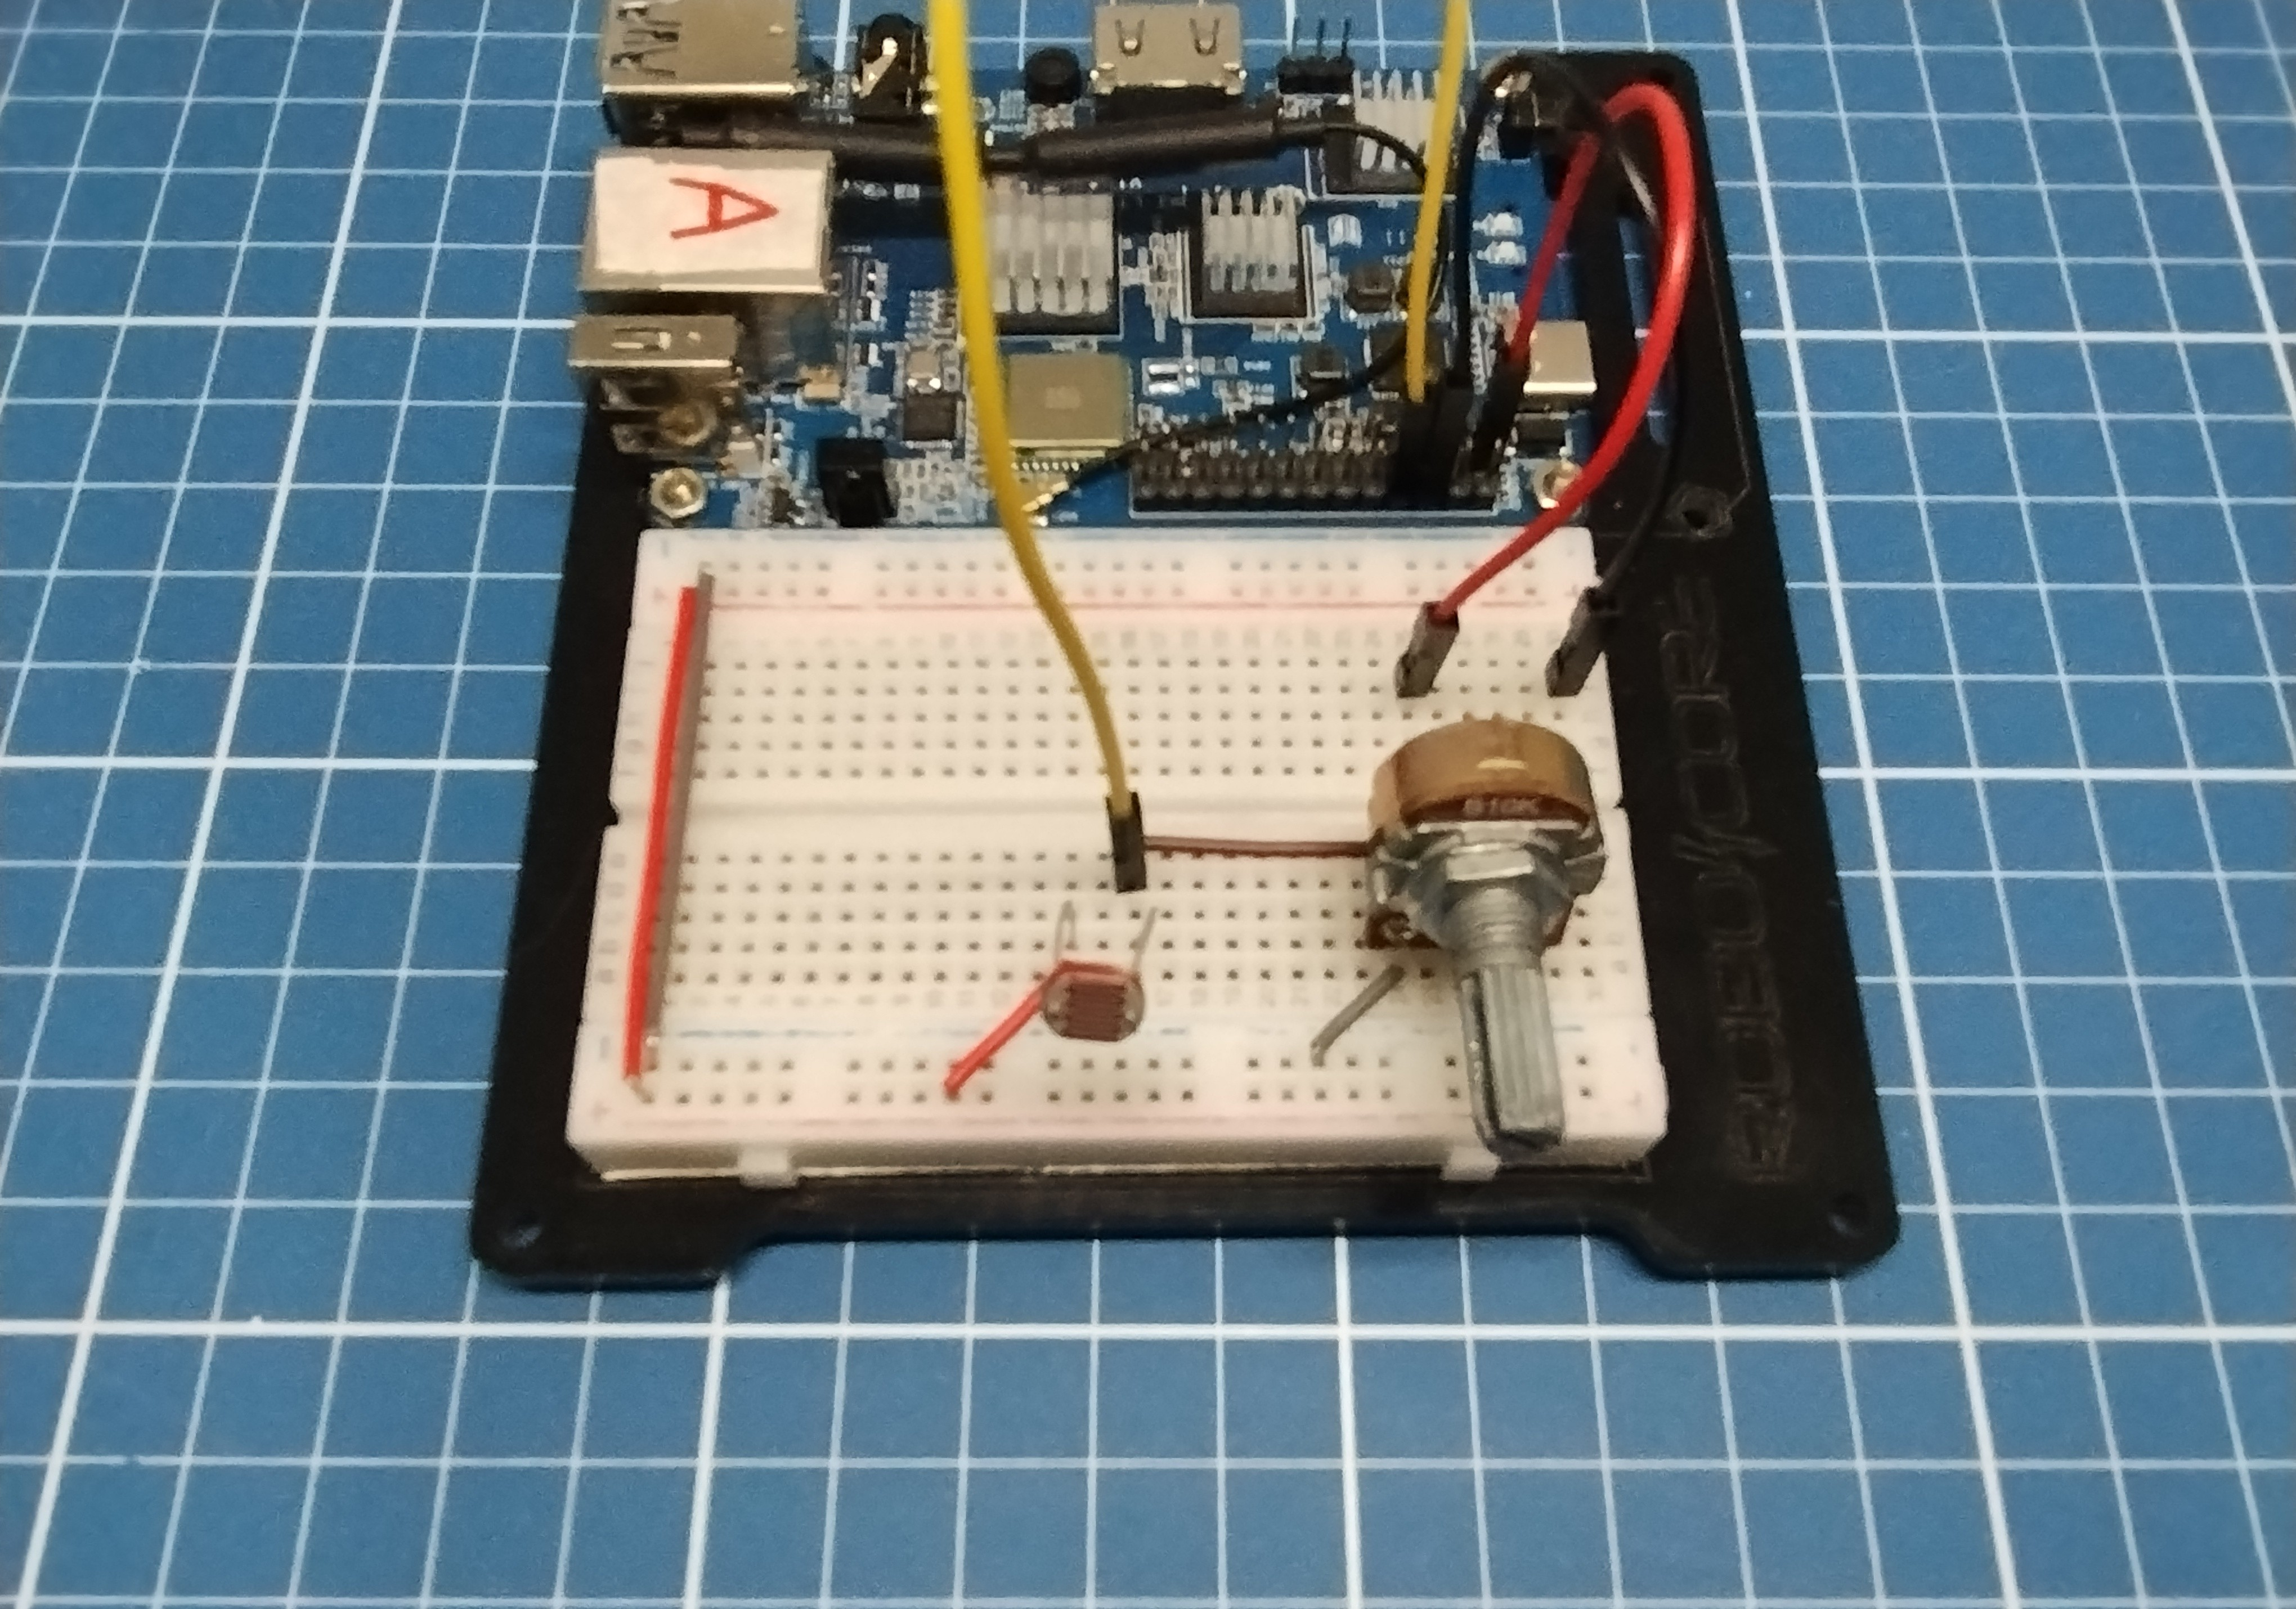
\includegraphics[width=0.4\textwidth]{images/foto_circuito_receptor.jpg}
  \legend{Fonte: Autor (2023)}
  \label{foto-circuito-receptor}
\end{figure}

\subsection{Software}

O código foi implementado nas SBCs usando a biblioteca \textit{wiringPi} e \textit{wiringOP}, que é um \textit{fork} da \textit{wiringPi} para a \textit{OrangePi}. O \textit{software} implementa um protocolo de comunicação chamado de \textit{start-stop}, que consiste em uma forma de sinalizar o iníco e o fim de uma transmissão de dados. No início, é eviado um bit de \textit{"start"} indicando o início da transmissão seguido dos dados e por fim um bit de \textit{"stop"} indicando o fim.



  % Referencias
  \bibliography{referencias}

\end{document}
